\documentclass{beamer}

\definecolor{OSUdkbrn}{RGB}{104,80,64}
\definecolor{OSUmedbrn}{RGB}{176,96,16}
\definecolor{OSUltbrn}{RGB}{224,195,152}
% from: http://oregonstate.edu/brand/color-palette

\mode<presentation>
{
	\usetheme{CambridgeUS}
	\setbeamercovered{transparent}
	\setbeamertemplate{footline}[page number]{}
	\setbeamercolor{palette tertiary}{fg=white, bg=OSUdkbrn}
	\setbeamercolor{title}{fg=OSUdkbrn}
	\setbeamercolor{frametitle}{fg=OSUdkbrn}
}

\title{Predicting Wine Quality: A Conundrum}
\subtitle{Would you like some cheese with that?}
\author{Kalbi Zongo, Song Hoa Choi, Gina Shellhammer, Matt Edwards}
\date{June 2, 2014}

\begin{document}
\begin{frame}
	\titlepage
\end{frame}

%\begin{frame}
%	\frametitle{Outline}
%	\tableofcontents
%\end{frame}

% -------------------------------- INTRODUCTION --------------------------------------------------
\section{Introduction}

\begin{frame}{Popping the Cork}
	\begin{figure}
		\centering
		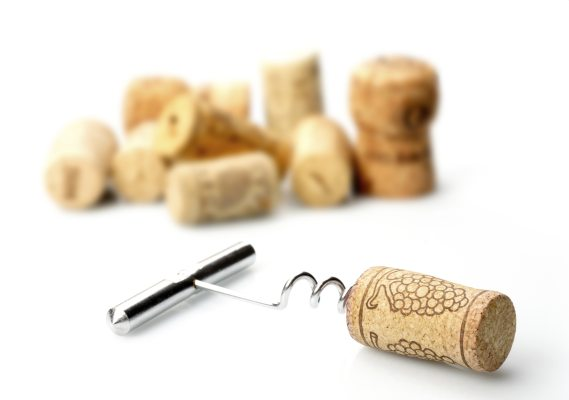
\includegraphics[width=\textwidth]{../images/uncork.jpg}
	\end{figure}
\end{frame}


\begin{frame}{Task}
	\LARGE
	\textbf{Predict} the blind taster quality score of a wine based on chemical tests.

\end{frame}

\begin{frame}{Data}
\begin{itemize}
	\item Two Datasets: Red \& White vinho verde wine samples from northern Portugal
	\item[]
	\item 1599 \& 4898 rows, respectively
	\item[]
	\item Concentrated on White Wine, due to more data
\end{itemize}
\end{frame}


\begin{frame}{Data}
\begin{itemize}
	
	\item 11 Explanatory variables: measurements from various phytochemicals in wine
	\item[]
	\item Response variable ``quality'' is discrete variable on ordered scale from 0 (worst) to 10 (best)
	\item[]
	\item Nothing graded as 0, 1, 2, or 10	
\end{itemize}
\end{frame}

\begin{frame}{White Wine Quality Scores}
\begin{figure}
	\centering
	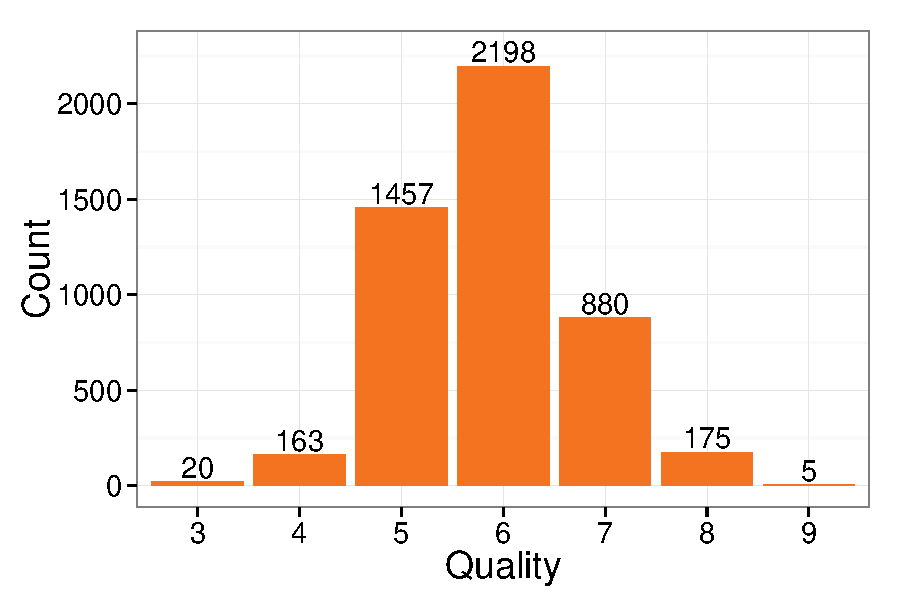
\includegraphics[width=\textwidth]{../images/white_hist.pdf}
\end{figure}
\end{frame}

% -------------------------------- MACHINE LEARNING METHODS --------------------------------------------------
\section{Machine Learning Methods}

\begin{frame}{Learning about Wine}
	\begin{figure}
		\centering
		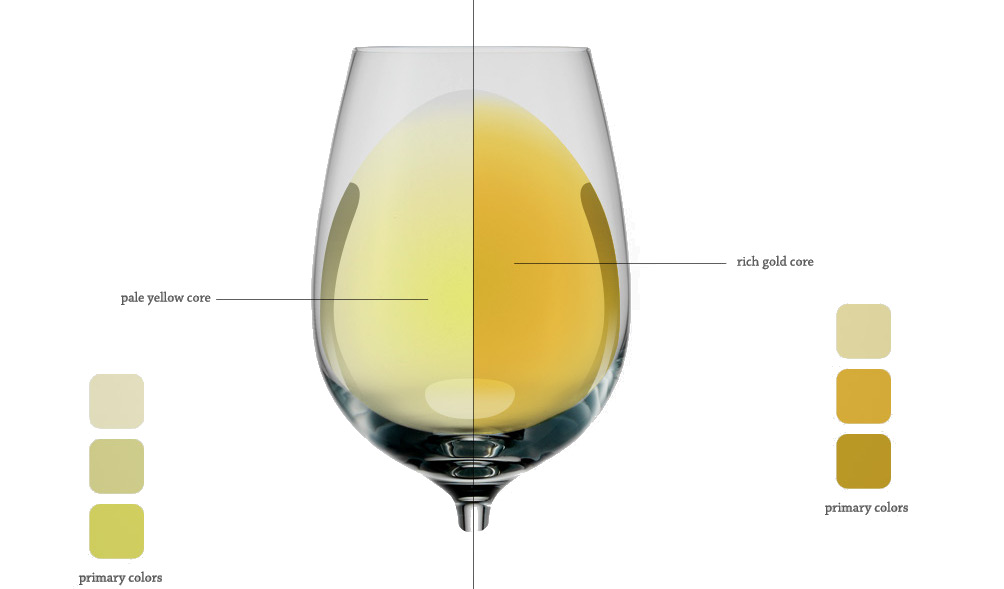
\includegraphics[width=\textwidth]{../images/matching.jpg}
	\end{figure}
\end{frame}

\begin{frame}{Training and Testing Sets}
	\begin{itemize}
	\item Training and Testing sets constructed through stratified sampling.
	\item[]
	\item Quality variable was the strata
	\item[]
	\item Why: Ensure representation of all quality categories in both Training \& Testing datasets.
	\item[]
	\item How: 37.5\% of items (rounded up) in strata were randomly selected to be in the testing set. Remaining 62.5\% were the training set.
	\item[]
	\item Regression and Random method used these training sets, Classification used different set.	
	\end{itemize}
\end{frame}

\begin{frame}{Methods}
	\begin{itemize}
	\item With ``prediction'' as the goal, we think regression.
	\item[]
	\item Forward, Backward and Subset Model Selection done, all resulted in same model.
	\item[]
	\item Classification Method can also be used to predict.
	\end{itemize}
\end{frame}



\begin{frame}{K-Nearest Neighbor Regression}
	\begin{itemize}
	\item Using some measure of distance, find nearest neighbors in dataset
	\item[]
	\item Order examples by increasing distance
	\item[]
	\item Find a ``optimal'' number $k$ of nearest neighbors
	\item[]
	\item Calculate an inverse distance weighted average with the $k$-nearest multivariate neighbors
	\item[]
	\item Used \texttt{fit} function from \texttt{rminer} package in R. Offers many regression types 
	\end{itemize}
\end{frame}


\begin{frame}{Ordinal Regression}
	Also ``Ordered Logistic'' Regression
	\begin{itemize}
	\item Estimate seperate binary regression models for all of: $P(score\leq j)/P(score>j)$, for all $j$
	\item[]
	\item To get the probability of the score being $j$: $P(Score=j)=P(score\leq j) - P(score < j)$
	\item[]
	\item So we can get the probability of each category.
	\end{itemize}
\end{frame}

\begin{frame}{Multiclass Classification}
	One-vs-All (or One-vs-Rest) Algorithm
	\begin{itemize}
%	\item Split data into training, cross-validation and test sets.
%	\item[]
	\item Split problem into $n$ binary classification problems, where $n$ is number of classes.
	\item[]
	\item Treat class $i$ as "positive" class, everything else as "negative" class
	\item[]
	\item Train logistic regression classifier $h_{\theta}^{i}(x)$ for each class $i$ to predict the probability that $y=i$
	\item[]
	\item On new input $x$, evaluate $\max_{i}h_{\theta}^{i}(x)$, so whichever class has the highest probability based on our input, we then predict $\hat{y}$ to be in that class
	\end{itemize}

%Logistic regression used as classifcation to predict category
\end{frame}

\begin{frame}{Random Randomness is Random}
	\begin{itemize}
	\item 75\% of Quality ratings were either 5 or 6. 
	\item[]
	\item Is randomly assigning 5 or 6 to everything as good as, or better than, our other methods?
	\item[]
	\item Using \texttt{rbinom(1,1,0.6014)}, 1s were predicted as quality 6, 0s as quality 5
	\item[]
	\item Probability of 60.14\% because from Training Set, considering only 5s and 6s, 6s were 60.14\% of total observations
	\item[]
	\item Our base line success rate to compare other methods.
	\end{itemize}
\end{frame}


% -------------------------------- FINDINGS --------------------------------------------------
\section{Findings}
\begin{frame}{Results}
	\begin{figure}
		\centering
		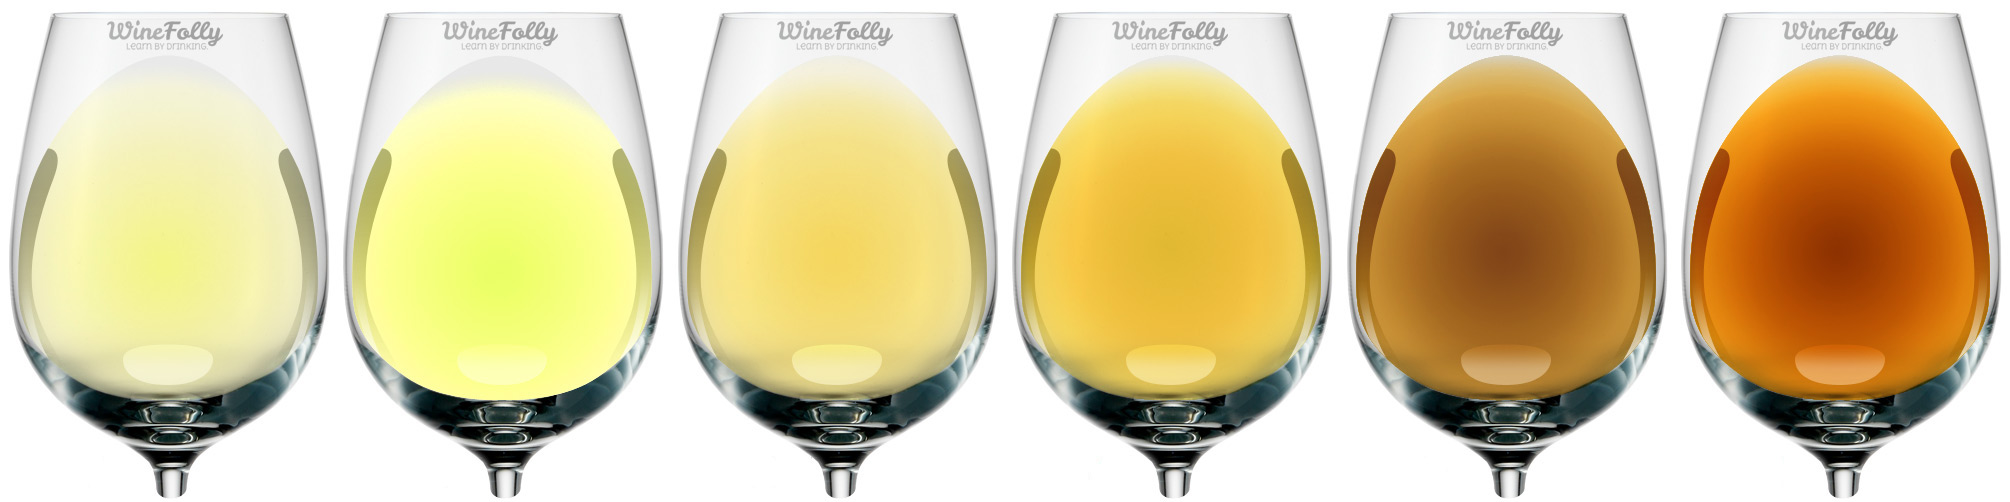
\includegraphics[width=\textwidth]{../images/gradient.jpg}
	\end{figure}
\end{frame}



\begin{frame}{K Nearest Neighbors Regression: 59.6\% Success Rate}
	\begin{figure}
		\centering
		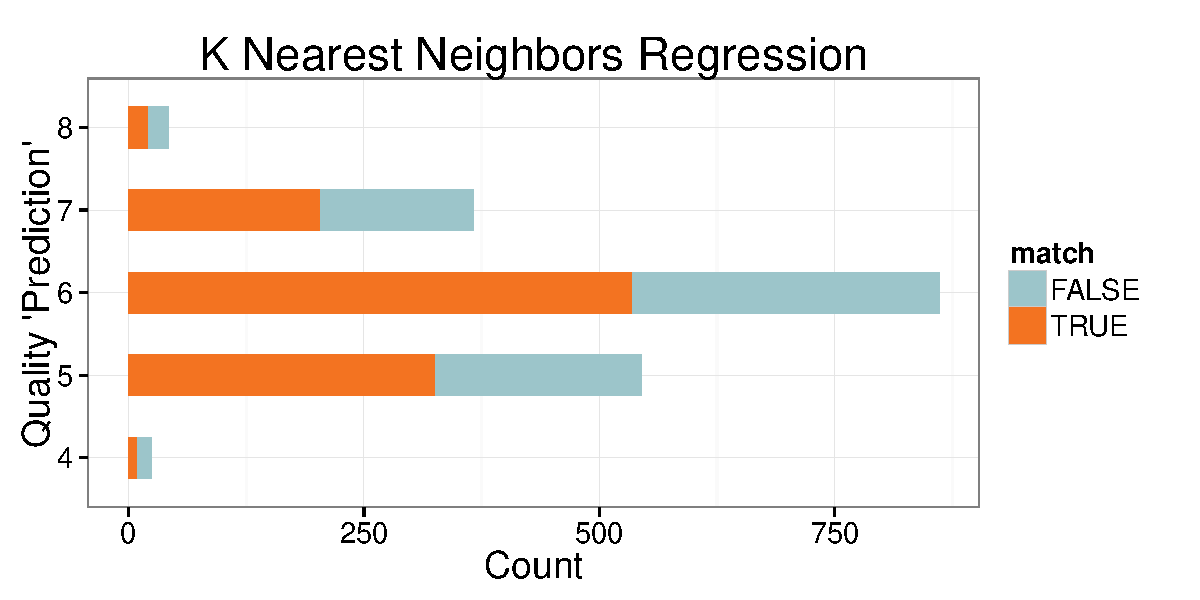
\includegraphics[width=\textwidth]{../images/KNNRegression_Results.pdf}
	\end{figure}

\end{frame}


\begin{frame}{Ordinal Regression: 53.3\% Success Rate}
	\begin{figure}
		\centering
		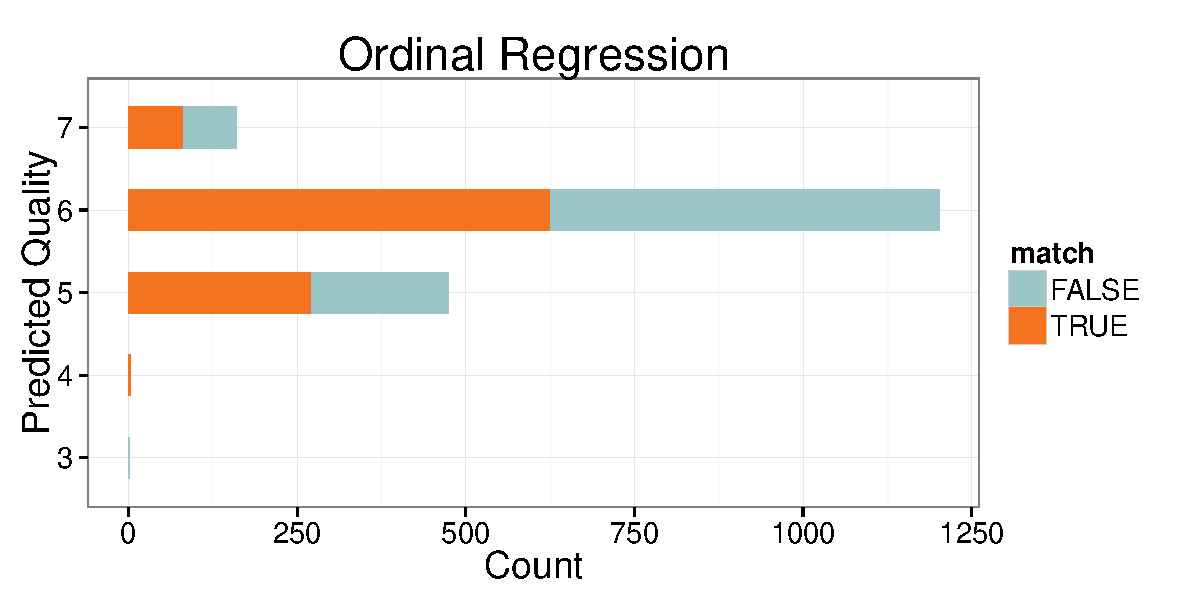
\includegraphics[width=\textwidth]{../images/OrdinalRegression_Results.pdf}
	\end{figure}

\end{frame}

\begin{frame}{Regression Summary}
	\begin{itemize}
	\item K Nearest Neighbors
	\begin{itemize}
		\item[]
		\item Overall 59.6\% success rate.
		\item[]
		\item No properly allocated 3s or 9s
	\end{itemize}
	\item[]
	\item Ordinal Regression
	\begin{itemize}
		\item[]	
		\item Overall 53.3\% success rate
		\item[]		
		\item No properly allocated 3s, 8s or 9s.
	\end{itemize}
	
	\end{itemize}

\end{frame}

%\begin{frame}{Regression: Success by Quality Predicted}
%\begin{center}
%
%\begin{tabular}{c | r r | r r | c}
%	           & \multicolumn{2}{c|}{KNN} & \multicolumn{2}{c|}{Ord} &  \\ \hline
%	Prediction & \% Match & \% Fail       & \% Match & \% Fail      & \# Present \\ \hline
%	    3      & n/a      & n/a           & 0\%      & 100\%        & 8         \\
%	    4      & 40.0\%   & 60.0\%        & 100\%    & 0\%          & 62        \\
%	    5      & 59.8\%   & 40.2\%        & 57.4\%   & 42.6\%       & 547       \\
%	    6      & 62.1\%   & 37.9\%        & 52.0\%   & 48.0\%       & 825       \\
%	    7      & 55.7\%   & 44.3\%        & 50.6\%   & 49.4\%       & 330       \\
%	    8      & 48.8\%   & 51.2\%        & n/a      & n/a          & 66        \\
%	    9      & n/a      & n/a           & n/a      & n/a          & 2
%\end{tabular}
%Success by predicted quality. `N/A' means nothing predicted at that quality.
%\end{center}
%\end{frame}




\begin{frame}{Classification: 54.4\% Success Rate}
	\begin{figure}
		\centering
		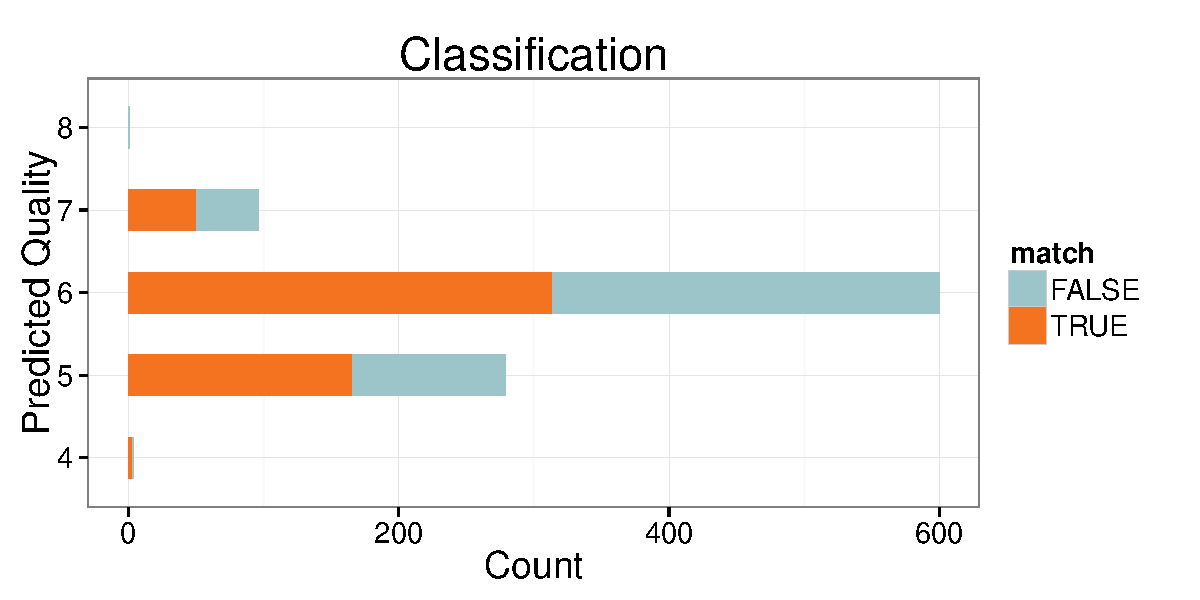
\includegraphics[width=\textwidth]{../images/Classification_Results.pdf}
	\end{figure}
\end{frame}

\begin{frame}{Classification Summary}
	\begin{itemize}
	\item 54.4\% success rate
	\item[]
	\item No properly allocated 3s or 9s
	\end{itemize}
\end{frame}

\begin{frame}{Comparison: Success by Quality Predicted}
	\begin{center}
	
	\begin{tabular}{c | r r | r r | r r|}
		           & \multicolumn{2}{c|}{KNN} & \multicolumn{2}{c|}{Ordinal} & \multicolumn{2}{c|}{Classification}          \\ \hline
		Prediction & \% Match & \% Fail       & \% Match & \% Fail       & \% Match & \% Fail       \\ \hline
		    3      & n/a      & n/a           & 0\%      & 100\%         & n/a      & n/a           \\
		    4      & 40.0\%   & 60.0\%        & 100\%    & 0\%           & 75.0\%   & 25.0\%        \\
		    5      & 59.8\%   & 40.2\%        & 57.4\%   & 42.6\%        & 59.5\%   & 40.5\%        \\
		    6      & 62.1\%   & 37.9\%        & 52.0\%   & 48.0\%        & 52.3\%   & 47.7\%        \\
		    7      & 55.7\%   & 44.3\%        & 50.6\%   & 49.4\%        & 52.1\%   & 47.9\%        \\
		    8      & 48.8\%   & 51.2\%        & n/a      & n/a           & 0\%      & 100\%         \\
		    9      & n/a      & n/a           & n/a      & n/a           & n/a      & n/a           \end{tabular}
	
	\end{center}
	`N/A' means nothing predicted at that quality.
\end{frame}

\begin{frame}{Random 'Prediction': 39.67\% Success Rate}
	\begin{figure}
		\centering
		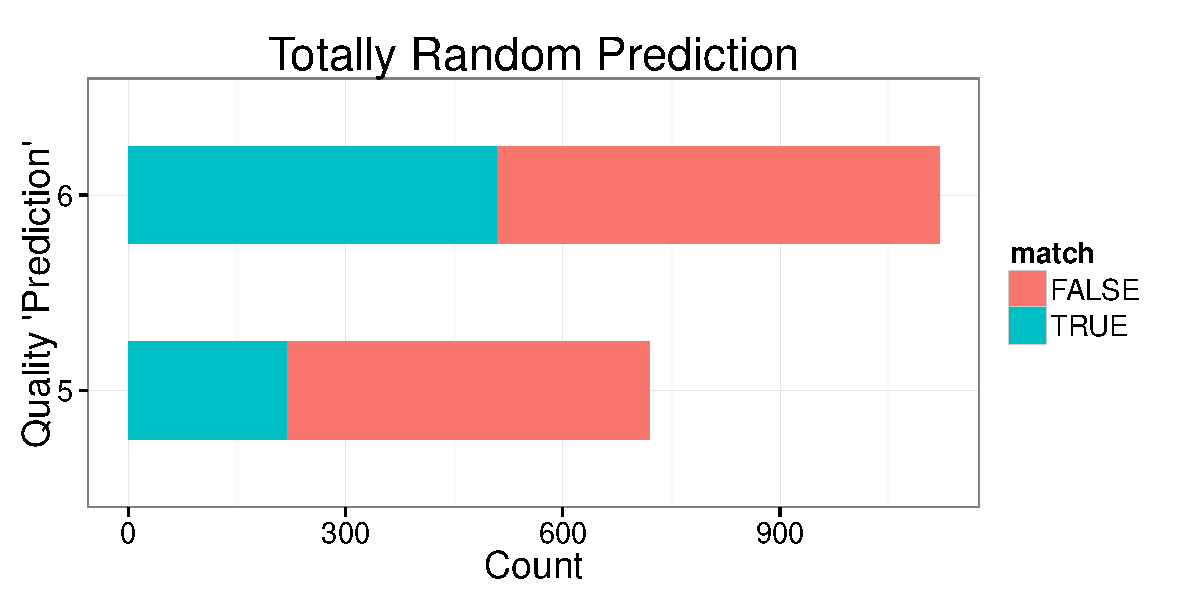
\includegraphics[width=\textwidth]{../images/RandomPrediction.pdf}
	\end{figure}
	Turns out, that's not really a great 'prediction' method. Who knew?
\end{frame}


% -------------------------------- DISCUSSION --------------------------------------------------
\section{Discussion}
\begin{frame}{Discussion}
	\begin{figure}
		\centering
		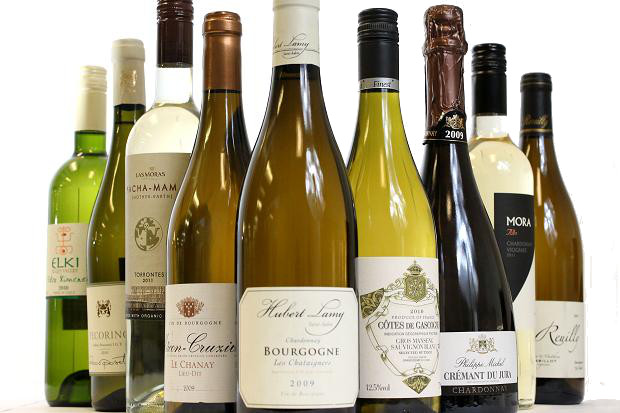
\includegraphics[width=\textwidth]{../images/wines.jpg}
	\end{figure}
\end{frame}

\begin{frame}{One-vs-All Classification: Assumptions}
	\begin{itemize}
	\item Need 3 data sets if doing Model Selection. 
	\item[]
	\item Assumes that the individual logistic regressions are independent, meaning that the probability of all categories do not sum to one. 
	\item[]
	\item Approach assumes that the category with higher probability is more likely to occur that other categories
	\end{itemize}
\end{frame}

\begin{frame}{One-vs-All Classification: Limitations}
	\begin{itemize}

	 \item When two or more categories have the same probability of success, then the approach will just pick one. 
	 \item[]
	 \item The algorithm is computationally expensive. Ran in about 3 mins for this data set.
	 \item[]
	 \item Scalability is an issue for the algorithm, larger data sets could cause issues.
	\end{itemize}

\end{frame}

\begin{frame}{Cross-Validation}
Lambda is tuning parameter for model. Want to pick the lambda with the lowest cross-validation. 

	\begin{figure}
		\centering
		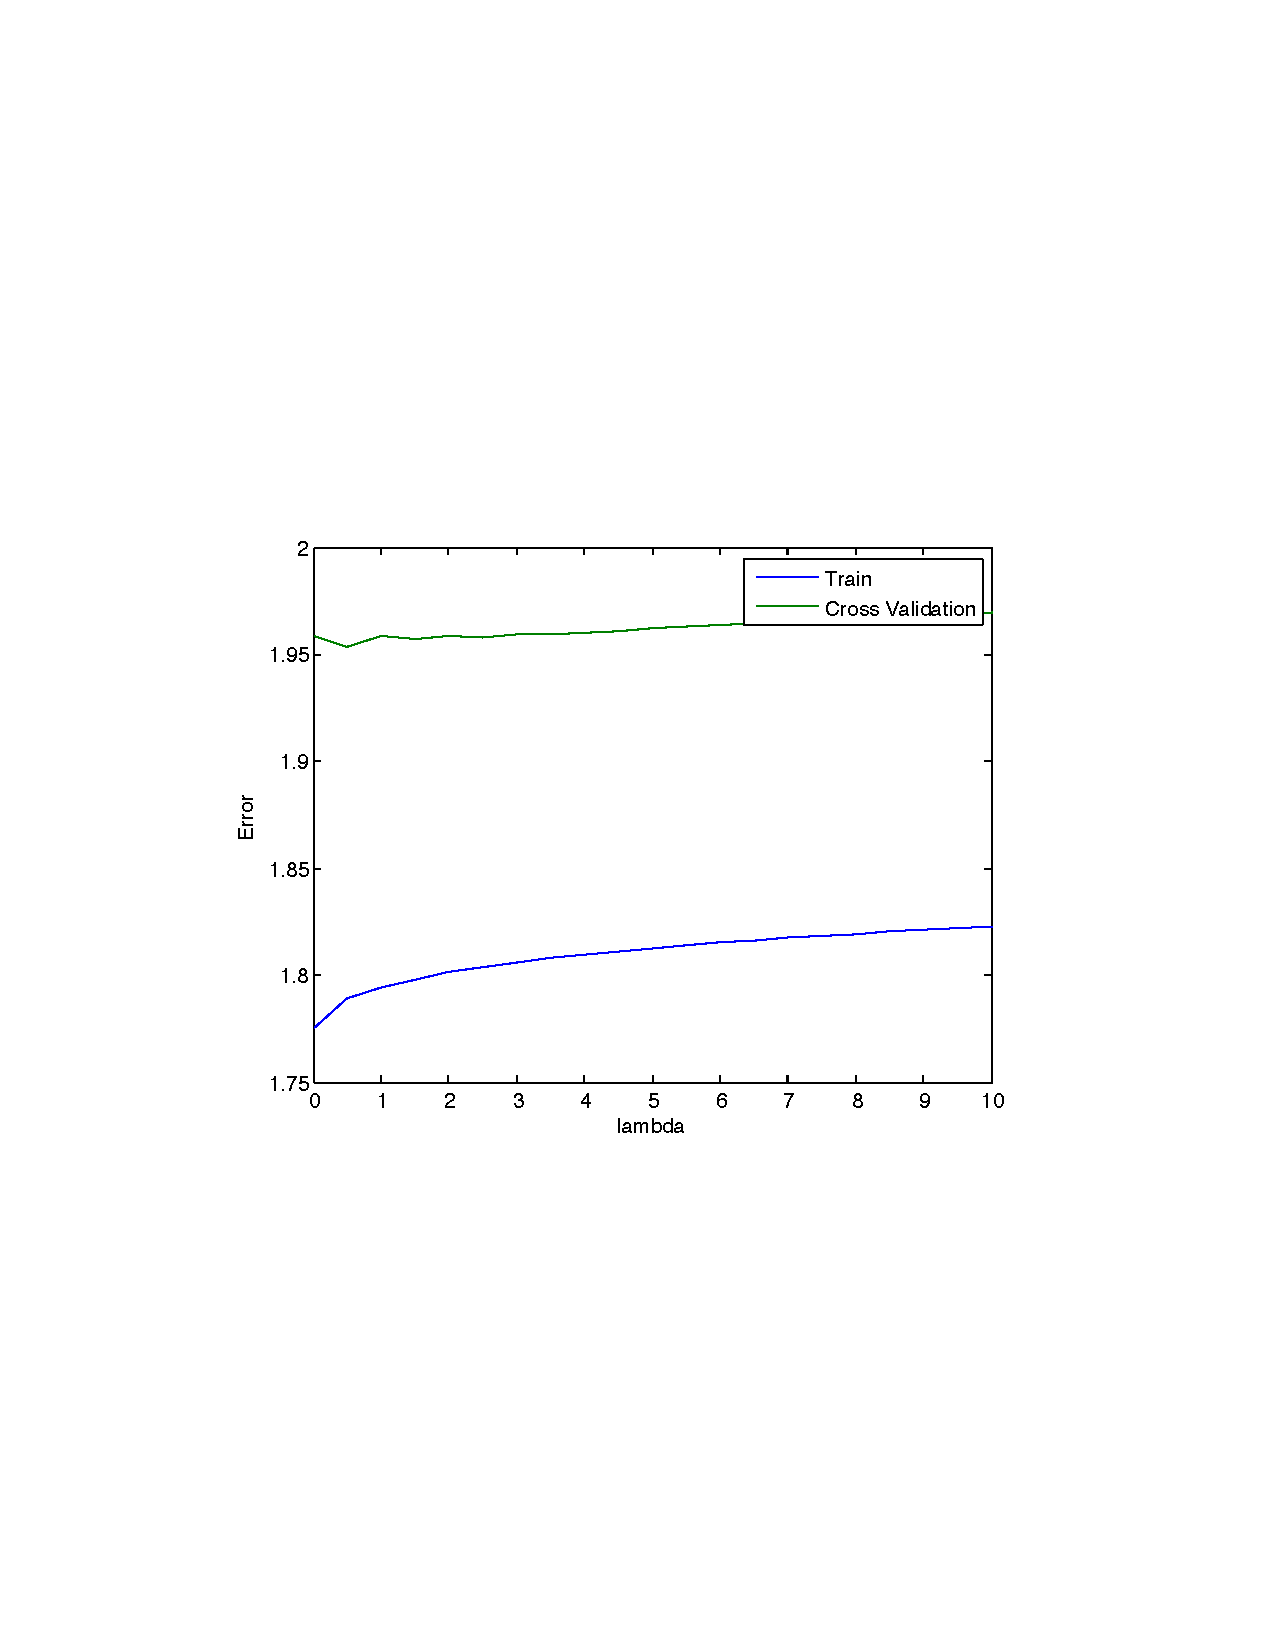
\includegraphics[scale=0.5]{../images/validationcurve.pdf}
	\end{figure}

\end{frame}


\begin{frame}{Regression: Assumptions}
	\begin{itemize}
	\item Multicollinearity is not an issue with prediction. It blows up SE, which is bad for estimation, not so bad with prediction.
	\item[]
	\item K-Neighbors: Options available for the ``search method'' for KNN algorithm were not explored. This changes how the hyper-parameters of the algorithm are tuned.
	\item[]
	\item Cross validation was not explored.
	\end{itemize}
\end{frame}

\begin{frame}{Ordinal Regression Assumptions}
	\begin{itemize}
	\item Because it is likelihood based, need to have ``enough'' data for modeling.
	\item[]
	\item Proportional odds - coefficients stay the same, and the intercept value changes. Need to verify. Did not do it.
	\item[]
	\item To verify, would run each category independently, verifying slopes are the same.
	\item[]
	\item All explanatory variables have the same weight for all categories. Puts them in possible categories, picks the one with the highest probability. 
	\end{itemize}
\end{frame}

\begin{frame}{Regression:Limitations and Scaling}
	\begin{itemize}
	\item K-Neighbors: if category distribution is skewed, larger categories can dominate, which is what we see in our results.
	\item[]
	\item Regression does not always scale well, adding covariates can bog down the number of comparisons, especially with model selection
	\item[]
	\item Random or stratified sampling of data to get a reasonable set size and model selection to cut down number of covariates could help.
	\end{itemize}
\end{frame}

\begin{frame}{Questions}
	\begin{figure}
		\centering
		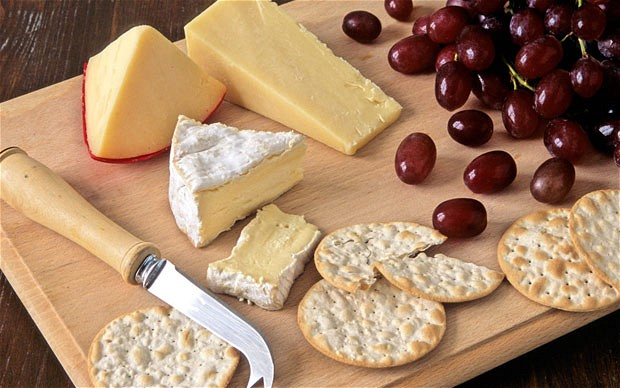
\includegraphics[width=\textwidth]{../images/cheese.jpg}
	\end{figure}
\end{frame}

\end{document}
